In the Heat Transfer algorithm~(HT), we have a graph where heat values are
exchanged between nodes. The goal of the program is to exchange heat to a point
where new heat value $\delta = |H_i -
H_{i-1}| \le \epsilon$ for all nodes of the graph. The algorithm works
asynchronously since heat values can be updated by using new partial information
coming from neighbor nodes. This increases parallelism since nodes do not need
to synchronize between iterations.

Fig.~\ref{code:ht} shows the HT logical rules that send new heat values to
neighbor nodes. In the first rule we added \texttt{add-priority} to increase the priority of the neighbor
nodes if the current node has a large $\delta$. The idea is to prioritize the
computation of heat values of nodes (using \texttt{update}) that have a neighbor
that changed significantly. Multiple \texttt{add-priority} facts will
increase the priority of a node so that nodes with multiple large deltas will
have more priority. To further improve scalability, we added the third rule to
ignore to not send small $\delta$ values if the target node is in another
thread. Note that the LM compiler will merge the three rules in
Fig.~\ref{code:ht} into a single one that handles the 3 branches.

\begin{topfig}
\scriptsize\begin{Verbatim}[numbers=left,commandchars=\\\[\]]
new-heat(A, New, Old),
Delta = fabs(New - Old),
Delta > epsilon
   -o {B, W | !edge(A, B, W) |
         new-neighbor-heat(B, A, New),
         update(B), \underline[add-priority(B, Delta)]}.

new-heat(A, New, Old)
fabs(New - Old) <= epsilon
\underline[cpu-id(A, B, C)],
\underline[cpu-id(A, A, C)]
   -o {B, W | !edge(A, B, W) |
         new-neighbor-heat(B, A, New)}.

new-heat(A, New, Old)
fabs(New - Old) <= epsilon,
\underline[cpu-id(A, B, C1)],
\underline[cpu-id(A, A, C2)],
\underline[C1 <> C2]
   -o 1. // nothing is derived
\end{Verbatim}
  \scap{code:ht}{Coordination code for the Heat Transfer program. We updated the first rule
     to increase the priority of neighbor nodes and added the third rule to not
     send small $\delta$ if the neighbor is in another thread. The code logic remains exactly
     the same as before, however bigger changes in heat values are now
     propagated faster.}
\end{topfig}
\normalsize

Fig.~\ref{results:ht} presents the scalability results for the uncoordinated
and coordinated version. The dataset used is a square grid with an inner square
with high heat nodes. With 1 thread, there's a 33\% reduction in run time, while
for 16 threads, there's a 18\% reduction.

\begin{topfig}
   \begin{center}
      \subfloat[]{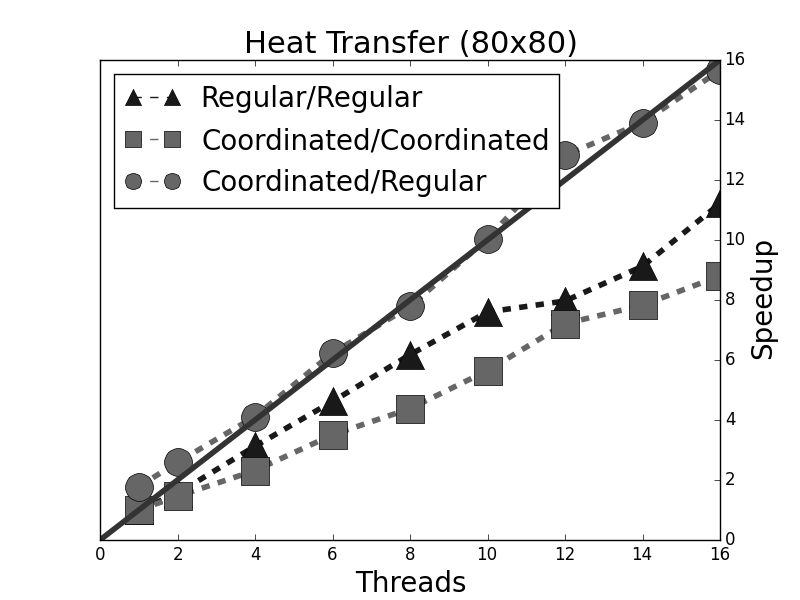
\includegraphics[width=5cm]{results/new-heat-transfer-80}}
   \end{center}
   \scap{results:ht}{Experimental results for the HT program. The coordinated version
      is, on average, 30\% faster than the regular version although it has a
      slightly worse scalability due to a reduction in work available.}
\end{topfig}
